% !TeX spellcheck = en_GB
\chapter{Supplemental figures}

\begin{figure}[ht]
	\centering
	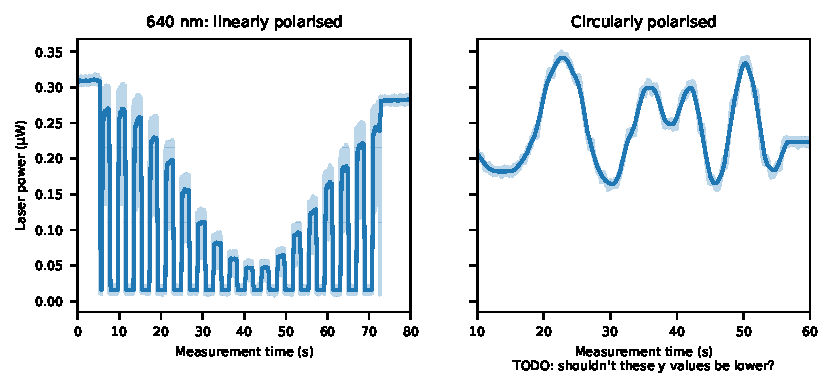
\includegraphics{640 laser pol characteristics in sample}
	\caption{
		Polarisation characteristics at the sample plane of the 640 laser. \textbf{Left:} power transmitted through a stationary polariser aligned to maximise transmission of the 640 laser set to an polarisation of 0° (vertical in the sample plane), while the laser beam rotates. \textbf{Right:} power transmitted through a manually rotating polariser, while the beam is set to circular polarisation.
	}
	\label{fig:640 laser pol at sample}
\end{figure}

\begin{figure}[ht]
	\centering
	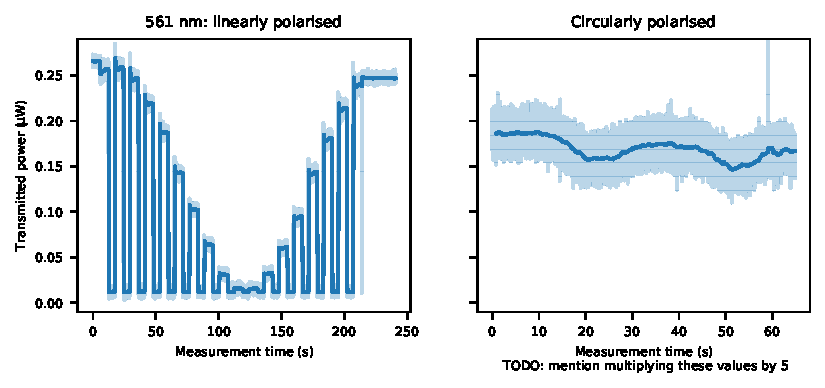
\includegraphics{561 laser pol characteristics in sample}
	\caption{
		Polarisation characteristics at the sample plane of the 561 laser. Left and right panes are the same as \autoref{fig:640 laser pol at sample}. (As the data on the left was acquired at 50\% laser power to increase the signal at minimum transmission, but the data on the right was acquired at 10\% laser power for safety reasons, the data on the right has been multiplied by a factor of 5 to allow comparison between the two figures. This also increased the noise.)
	}
	\label{fig:561 laser pol at sample}
\end{figure}

\begin{figure}[ht]
	\centering
	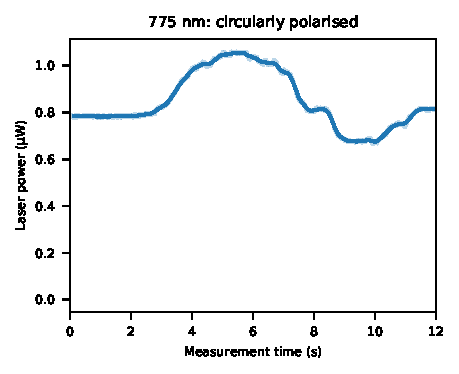
\includegraphics{775 laser pol characteristics in sample (donut beam, no psted optics)}
	\caption{
		Polarisation characteristics at the sample plane of the depletion beam, without pSTED optics. As its polarisation state cannot be manipulated through the software, only circular polarisation is characterised by manually rotating a polariser at the sample plane and measuring the transmitted power.
	}
	\label{fig:775 laser pol at sample}
\end{figure}

\begin{figure}[ht]
	\centering
	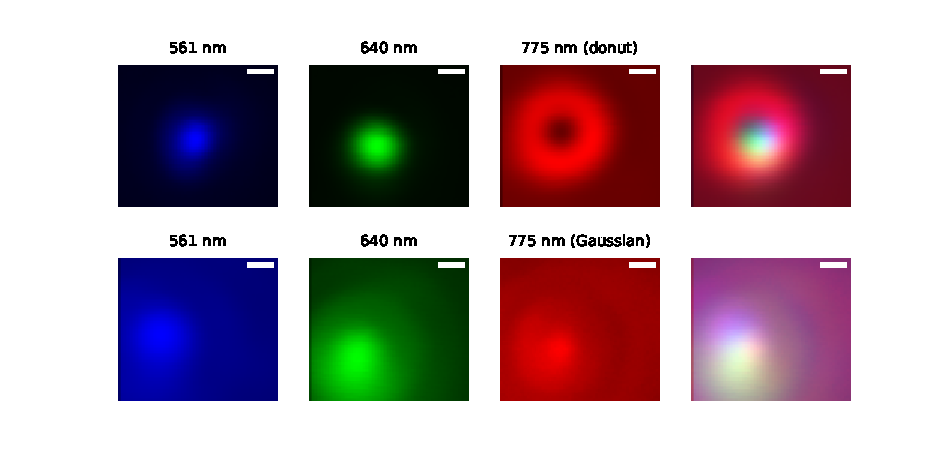
\includegraphics{laser_psfs.pdf}
	\caption{
		Point spread functions of the different lasers at different SLM configurations, by measuring the reflection from 100 nm wide gold beads. Scale bars 200 nm. \todo{show better data from 26 march}
	}
	\label{fig:normal psfs}
\end{figure}

\begin{figure}[ht]
	\centering
	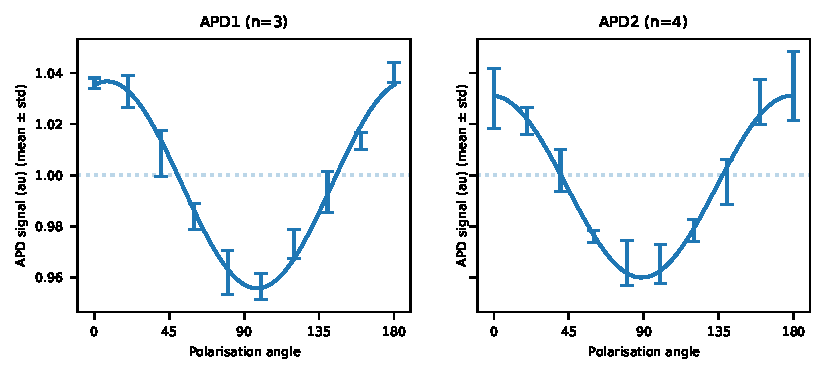
\includegraphics{apd_pol_sensitivity.pdf}
	\caption{Dependence of the signal from APD1 on the angle of polarisation of incoming light.}
	\label{fig:apd pol sensitivity}
\end{figure}


\begin{figure}[ht]
	\centering
	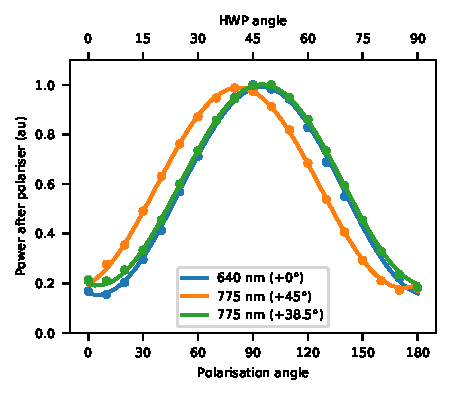
\includegraphics{psted_hwp_offset.pdf}
	\caption{
		The rotating HWP I put in the beamline controls the depletion beam polarisation. With an offset of 38.4°, the depletion beam is parallel to the 640 laser (set to vertical linear polarisation).
	}
	\label{fig:psted hwp offset}
\end{figure}